\documentclass{article}
\usepackage[utf8]{inputenc}
\usepackage{fontspec}
\usepackage{tabularx}
\usepackage{bbding}
\setmainfont[
  Path = ./,
  Ligatures = TeX,
  BoldFont = SABONLTSTD-BOLD.OTF,
  ItalicFont = SABONLTSTD-ITALIC.OTF,
]{SABONLTSTD-ROMAN.OTF}
\usepackage{book-of-common-prayer}
\geometry{
  paperheight=8.5in,
  paperwidth=5.5in,
  heightrounded,
}

\newwrite\dimensionout
\immediate\openout\dimensionout=linewidth.txt
\immediate\write\dimensionout{\the\linewidth}
\immediate\closeout\dimensionout

\title{
  \Large A Collection of\\
  \LARGE Private Devotions
}
\author{The Rt. Rev. John Cosin}
\date{}

\begin{document}

\begin{titlingpage}
  \begin{center}
    \thetitle \\
    \vspace{0.5cm}
    \begin{figure}[!htpb]
      \centering
      \vspace{2mm}
      \framebox{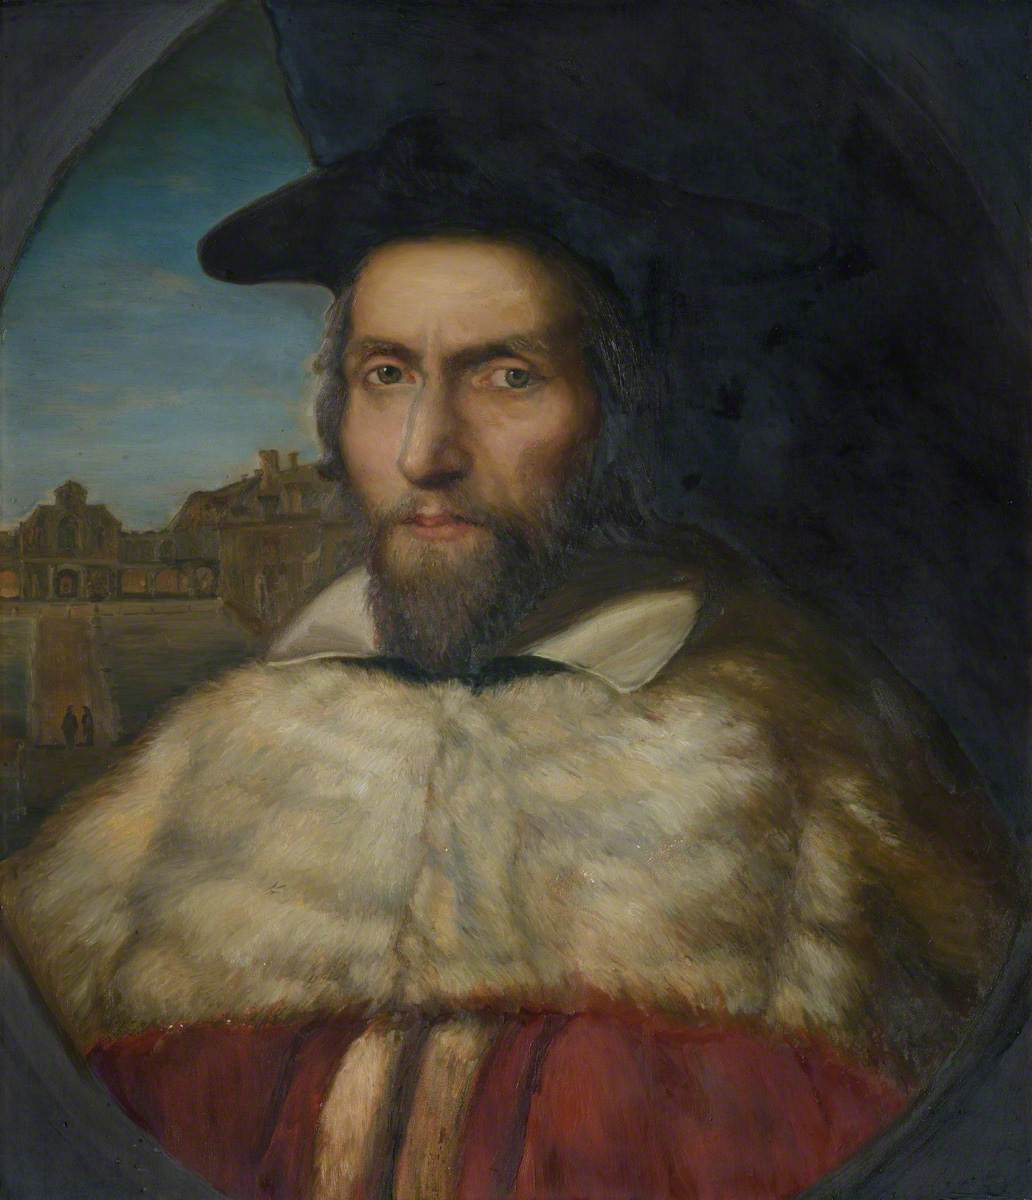
\includegraphics[scale=0.14]{images/John_Cosin_Peterhouse.jpg}}
    \end{figure}
    \theauthor \\
    \vspace{0.2cm}
  \end{center}
\end{titlingpage}

\newpage

\tableofcontents
\newpage

\section{Editor's Preface}

This is a fun little project of transcribing some of the Rt. Rev. John Cosin's
prayers. I've tried to make spelling consistent, and add helpful
remarks (noted with *). Additional sections to break up the text are introduced as well.
Likewise, erroneous capitalizations in the following are brought into
comformity with
our norms.

\newpage

\section{Preface}

For the good and welfare of our souls, there is not in Christian
religion any thing of like continual rule and force throughout
ever hour of our lives, as is the ghostly excercise of prayer
and devotion. Which the holy Apostles observing their
Lord and Master to frequently to use, in the Morning
(Mark 1:35) before day, in the Evening (Matthew 14:23)
before night, and otherwise to spend the whole night
in prayer (Luke 6:13), accounted it their duty
also to be followers of his example and practice,
as being a matter of high importance, and great benefit
thereby to be obtained.

And therefore they addressed themselves to Him, desiring him to teach them how
to pray, as S. John the Baptist had also taught his disciples. For which end
and purpose, our Saviour taught and prescribed  them a form
of prayer so absolute and so perfect as never was like made before; which,
from him who made it then, was ever afterward called the Lord's
Prayer (Luke 11:2; Matthew 6:9).

A prayer, whereby we have not only Christ's name to countenace our suits,
(in whole name if we wask anything, as we ought to do, he hath offered us in his
holy Gospel, that we should obtain it [John 16:23];) but Christ's
own word also, who himself is our Advocate (1 John 2:1), and being best
acquainted with the laws and phrases of his Father's court, hath both
for matter and form,
drawn up such supplications for us as will be most available and prevalatn
with Almighty God. And though Men should speak with angels tongues, yet words
that sill be more pleasing to the ears of God than those which the Son of God
did compose cannot possibly be uttered; nor can any prayers be so
well frameda s those that
are made by his blessed pattern.

It is for this cause called by the Father, The Prayer of all
Prayers\footnote{Augustine, \textit{Sermon 2 Post Pentecost};
Tertullian, \textit{De Oratio}, ch. 9}, and the rule or square
whereby all our petitions are to be formed; having likewise been
thus used in all ages of the Church, not only as a common part
of her prayers and service, but as the chief and fundamental part of them,
the ground whereupon she builds, the pattern whereby she frames,
and the complement wherewith she perfects all the rest of her
heavenly devotions,
framing them as this is framed, with much efficacy, though not with superfluity
of words.

Thus we begin at this day all our church services with the Lord's Prayer,
and lay it as a foundation whereon to build the rest of our petitions
that follow, sometimes continuing (as after the Creed) and sometimes perfecting
(as after the Blessed Sacrament) our most holy devotions with it:
thereby supplying with the fulness of that one, whatsoever may be
defective in all other
prayers, \textit{praemissa legitima oratione} (saith Tertullian)
\textit{quasi fundamento accidentium}, etc. (\textit{This is the law
    we go by, the groundwork and guide of all those holy prayers that
Christians use to make}).

A part of which ancient piety are these daily devotions and prayers
that hereafter follow;
prayers which, after the manner and division of
hours as they are\footnote{\textit{Horarium Regia authoritate editium}, etc. The
  Horary set forth with the Queen's authority (1560) and renewed
(1573). Imprinted with privilege at London by William Seers.},
having heretofore been purblished among us by high and sacred authority, are now
also renewed, and more fully set forth again, as for many other, so
chiefly for these
four reasons.

1. The first is, to continue and preserve the authority of the
ancient laws, and old
godly canons of the Church, which were made and set forth for this
purpose, that men,
before they set themselves to pray, might know what to say, and
avoid, as near as might be,
al extemporal effusions of irksome and indigested prayers, which they
use to make, that herein
are subject to no good order or form of words, but pray both what,
and how, and when they list.
Therefore among the ecclesiastical laws made in the time of Carolus
[Magnus Charlemagne],
we find this to be one; \textit{orationes, quae ab Ecclesia probatae,
non sunt rejiciantur}
(\textit{let no prayer be used but those which are allowed by the
church})\footnote{Microl. de Eccles. obser. cap. 4}
[Likewise], \textit{quascunque sibi preces aliquis describit, non eis
  utatur nisi prius
eas cum instructioribus contulerit} (\textit{what prayers soever any
    man hath framed
    for himself, let him first acquaint those that are wise and
    learned with them, before he presumeth
to use them})\footnote{Council of Carthage, Can. 23}.

And the reason is given in the 12th Canon of the Milevitan Council,
which was also
repeated in the 70th Canon of the Council of Alfric, \textit{ne forte aliquid
contra fidem, vel per ignorantiam vel per minus studium, sit compositum}
(\textit{let either through ignorance, or through less care than is
    fit, any thing be said
which is not consonant to the faith of Christ's Church}).

And that men may not think these rules are to be applied to public prayers only,
and not to private; let them weigh those words in the Council of Carthage,
\textit{quascunque sibi preces, etc.} (\textit{the prayers which a
    man makes for himself,
etc.}). And let them consider, that when Christ had bidden us to
enter into our chamber and pray
privately, presently he sets us a form to pray by even there in
secret (Matthew 6:6, 9).
By which passages those prayers are chiefly allowed and recommended
unto us, (for all
sudden and godly ejaculationsare not to be condemned) which with good
advice and meditation are framed
beforehand by them that best know what belongs thereunto: That so
through this means the worthiest
part of our Christian duty to God-ward might suffer no such scandal
and disgrace as otherwiles
it is forced to do; and that when we speak to our call upon the awful
majesty of Almighty God,
we might be sure to speak in the grave and pious language of Christ's
Church, which
hath evermore been guided by the Spirit of God and the Holy Ghost;
and not to lose our
selves with the confusion in any sudden abrupt or rude dictates,
which are framed
by private spirits and ghosts of our own. In regard whereof our very
priests and deacons
themselves are for their private and daily prayers enjoined to say the
morning and evening devotions of the Church \footnote{Preface before
  the [Book of Common Prayer:] \textit{All Priests and Deacons shall be
    bound daily to say the Mattins and Even-song, either openly or
  privately}: as it was of old ordained in the Council of Venice under
Leo the First, Can. 14., and in the Council of Mentz, Can. 57}; and when
at any time they pray, or bid the prayers before their sermons, ther
eis a set form of words
prescribed for them to use\footnote{Injunctions, capult. and Can. 55
in the Book of Canons and Constitutions Ecclesiastical.},
that they also might know, it is not so lawful for them to pray of
their own heads, or suddenly to say
what they please themselves.

2. The second is, to let the world understand that they who give it out, and
accuse us here in England to have set up a new Church and a new
faith\footnote{Sanders,
  [\textit{De origine ac progressu schismatis Anglicani}; ] Calvin.
  Turcis. [?; ]
  Brist Demon. [?; ] Certain [Articles] or forcible Reas. Art. 1.[; ]
  and the common
conceit of the most reluctatnt [Catholics].}, to have bandonded all the ancient
forms of piety and devotion, to have taken away all the religious exercises and
prayers of our fore-fathers, to have despised all the old ceremonies,
and cast behind us the blessed Sacraments of Christ's Catholic Church:
that these men do little else but betray their own infirmities, and
have more violence
and will that reason or judgment for what they say; the common accusations
which, out of the avundance of those partial affections that
transport them the wrong way,
they are pleased to bring so frequently against us, being but the
bare reports of
such people as either do not or will not understand us what we are.

3. The third is, that they who are this may already religiously
given, and whom earnest letts
and impediments do often hinder from being partakers of the public,
might have here a daily
and devout order of private prayer, wherein to exercise themselves,
and to spend some hours of the day
at least (as the old godly Christians were wont to do) in God's holy
worship and service; not
employing themselves so much to talk and dispute as to practice
religion, and to live like Christians:
the continual and curious disquisitions of many unncessary questions
among us being nothing else but either
the new seeds or the old fruits of malice, and by consequence the
enemy of godliness, and the abatement
of that true devotion wherewith God is more delighted, and a good
soul more inflamed and comforted,
than with all the busy subtilties of the world. In which sense Saint
[Augustine] was wont
to say, that the pious and devout, though unlearned, went to Heaven,
while other men,
trusting to their learning, disputed it quite away\cite{S. Aug.
  \textit{Veniunt indocti \& rapiunt coelum}: \& \textit{nos cum
doctrinis nostris detrudimur ad infernum.}}.

4. The last is, that those who perhaps are but codly this way yet
affected, might
by others eample be stirred up to the like heavenly duty of
performing their daily and Christian
devotions to Almighty God, as being a work of all others the most
acceptable to his Divine Majesty.

In doing so we shall all give evident testimony to the world whose
servants we are,
and wherein our chifest delight doth consist; we shall enjoy a
perpetual communion with all the saints triumphant
as well as militant, and we shall have just cause to conceive, that
so much of our life is celestial and divine
as we spend in this holy exercise of prayer and devotion.

\newpage
\section{The Compline}

\instruct{*First is read the following}

\bibleverse
{I will not suffer mine eyes to sleep, nor mine eye-lids to slumber,
  nor the temples of my head to take any rest, until I find out a place for the
habitation of the Lord.}
{Psalm 132:4}

\bibleverse
{Tell me, with what confidence canst thou lie down to sleep, and pass away
  the black darkness of night? With what fearful and ugly dreams shall thy
  soul (thinketh thou) be troubled, unless thou shalt first arm thyself against
  such delusions and fears, by strong and devout prayer? Let the wicked spirits
  find thee without such a guard, and presently thou becomest a prey
  unto them. Let them
  but spy thee at thy prayers, and presently, like frighted thieves,
they ran away.}
{St. John Chrysostom, I. \textit{De Orando Deum}}

\subsection*{The Psalm}

\instruct{*Then is said the following Antiphon and Psalm}

\textbf{The Antiphon}: \textsc{God} be merciful unto us, and bless
us: and shew us the light
of his countenance and be merciful unto us.

\textbf{Psalm 91:1-6}: \textit{Qui habitat}

\instruct{To be said at this time according to the direction of the
Rule of St. Basil}

\begin{enumerate}[
      leftmargin=*,
      label=\textsc {\arabic *}
    ]
  \item \psalmverse{Whoso dwelleth under the defence of the Most High:}
    {shall abide under the shadow of the Almighty.}
  \item \psalmverse{I will say unto the \textsc{Lord}, Thou art my hope, and
    my stronghold:} {my God, in him will I trust.}
  \item \psalmverse{For he shall deliver thee from the snare of the
    hunter:} {and from the noisome pestilence.}
  \item \psalmverse{He shall defend thee under his wings, and thou
    shalt be safe under his feathers:} {his faithfulness and truth
    shall be thy shield and buckler.}
  \item \psalmverse{Thou shalt not be afraid for any terror by
    night:} {nor for the arrow that flieth by day.}
  \item \psalmverse{For the pestilence that walketh in darkness:}
    {nor for the sickness that destroyeth in the noon-day.}
  \item[] \psalmverse{Glory be to the Father, and to the Son,}
    {and to the Holy Ghost.}
  \item[] \psalmverse{As it was in the beginning, is now, and ever shall be:}
    {world without end. Amen.}
\end{enumerate}

\subsection*{The Lesson}

\instruct{*Then is read the following brief lesson}

\bibleverse
{Be sober and watch, because your adversary the Devil goeth about
like a roaring lion, seeking whom he may devour. And the day of the Lord
will come as a thief in the night, in which the heavens shall pass away
with a great noise, and the elements shall melt with fervent heat. Seeing
then that all these things shall be dissolved, what manner of persons
ought we to be in in all holy conversation and godliness?}
{1 Peter 5:8; 2 Peter 3:10-11}

\subsection*{The Song of Simeon}

\instruct{*Then is sung or said the following Song of Simeon, or the Nunc Dimittis}

\begin{enumerate}[
      leftmargin=*,
      label=\textsc{\arabic *}
    ]
  \item \psalmverse{\textsc{Lord, now} lettest thou thy
    servant depart in peace:}
    {according to thy word.}

  \item \psalmverse{\textsc{For mine} eyes have seen thy salvation:}
    {which thou hast prepared before the face of all people;}

  \item \psalmverse{\textsc{To be} a light to lighten the Gentiles:}
    {and to be the glory of thy people Israel.}

  \item[] \psalmverse{\textsc{Glory} be to the Father, and
    to the Son:}
    {and to the Holy Ghost.}

  \item[] \psalmverse{\textsc{As it was} in the beginning, is now,
    and ever shall be:}
    {world without end. Amen.}
\end{enumerate}

\newpage
\subsection*{The Creed}

\instruct{*Then is said or sung the Apostle's Creed}

\begin{tabularx}{\linewidth}{lX}

    & I believe in God the Father Almighty, \\
    & maker of heaven and earth: \\
    & \\
    & And in Jesus Christ his only Son our Lord, \\
    & who was conceived by the Holy Ghost, \\
    & born of the Virgin Mary, \\
    & suffered under Pontius Pilate, \\
    & was crucified, dead, and buried. \\
    & He descended into hell; \\
    & the third day he rose again from the dead; \\
    & he ascended into heaven, \\
    & and sitteth on the right hand of God the Father Almighty; \\
    & from thence he shall come to judge the quick and the dead. \\
    & \\
    & I believe in the Holy Ghost; \\
    & the holy catholic church; \\
    & the communion of saints; \\
    & the forgiveness of sins; \\
    & the resurrection of the body, \\
    & and the life everlasting. \\
    & Amen.


\end{tabularx}

\subsection*{Kyrie and Lord's Prayer}

\instruct{*Then is said the Kyrie and Lord's Prayer}

\begin{tabularx}{\linewidth}{lX}

    & Lord, have mercy upon us. \\
    & \textit{Christ, have mercy upon us.} \\
    & Lord, have mercy upon us. \\
\end{tabularx}

\begin{tabularx}{\linewidth}{lX}
    & Our Father, who art in heaven, \\
    & hallowed be thy Name; \\
    & thy kingdom come; \\
    & thy will be done; \\
    & on earth as it is in heaven. \\
    & Give us this day our daily bread. \\
    & And forgive our trespasses, \\
    & as we forgive them that trespass against us. \\
    & And lead us not into temptation; \\
    & but deliver us from evil. Amen. \\
\end{tabularx}

\instruct{*After which is said:}

\textsc{The day} is thine, and the night is thine. Thou art 
worthy, O Lord, to receive honour, and praise, and worship
for evermore.

\subsection*{The Prayers}

\instruct{*One or more of the following collects is said}

Merciful Lord, who of thine abundant goodness towards us, hast
made the day to travel in, and ordained the night wherein to take our rest:
grant us such rest of body, that we may continually have a waking soul,
to watch for the time when the lord shall appear to deliver us from this mortal life.
Let no vain or wandering fancy trouble us: let our ghostly enemy have no power over us,
but let our minds be set wholly upon thy presence, so love, and fear, and rest in thee
alone: that being refreshed with a moderate and sober sleep, we may rise up again
with cheerful strength and gladness to serve thee in all good works,
through Jesus Christ our Lord. Amen.

\instruct{or}

Lighten our darkness, we beseech thee O Lord, and by thy great
mercy defend us from all perils and dangers of this night, for the love thy only Son,
our Saviour Jesus Christ. Amen.

\subsection*{The Benediction}

\instruct{*The final blessing is then said}

God the Father bless me: God the Son defend me: God the Holy Ghost
preserve me now and for ever. Amen.

\newpage
\section{Prayer at Bedtime}

\instruct{An admonition before we go to sleep}

\begin{prayer}

  Permit me not slugghis sleep,
    To close your waking eye,
  'Till that with judgment deep
    your daily deeds you try.
  He that his sins in conscience keeps
    when he to quiet goes,
  More desperate is than he that sleep
    amidst his mortal foes.

\end{prayer}

\instruct{When we enter into our Bed.}

In the name of the Lord Jesus Christ, who was crucified upon his cross
and laid into his grave for me, I lay me down to rest. He bless me,
keep me, and save me, raise me up again, and bring me at last to life
eternal. Amen.

\instruct{As we lay down to sleep}

\begin{prayer}

  At night lie down,
    prepare to have,
  Thy sleep thy death;
    thy bed thy grave.
  Awake, arise;
    think that thou hast
  Thy life but lent,
    thy breath a blast.

\end{prayer}

\subsection*{Final Prayers}

\instruct{*One or more of these final prayers is said before sleep}

I will lay me down in peace, and take my rest: for it is thou, Lord, only that makest me dwell in safety. Amen.

\instruct{or}

Have mercy upon me, O Lord, now, and at the hour of death. Amen.

\instruct{or}

O reserve me while I am waking, and defend me when I am sleeping, that my soul
may continually watch for thee, and both body and soul may rest in thy peace for ever.
Amen.

\end{document}
